\chapter{Health, Load, and the Co-Founder}

The interview begins with a narrow practical question: what steps did the founder learn to take in order to protect personal and mental health? The answer does not become a theory of wellness. It moves in a smaller and more useful order. First comes exercise, the obvious answer that is still true. Then comes the difficulty: exercise is precisely the thing a busy founder tends to sacrifice. Finally the answer becomes structural. A trusted co-founder changes the load-bearing design of the company.

\section{The Opening Question}

The question is framed as something learned ``during that process.'' That matters. We are not being handed a slogan from outside the work; we are being asked what survived contact with building a company.

The first object in the discussion is the founder under pressure. There is a business to build, meetings to attend, work to divide, and a personal life that can still produce emergencies. The problem is not simply that founders forget to care for themselves. The problem is that the business creates repeated incentives to treat self-care as movable.

\begin{definition}
In this chapter, a \emph{fungible commitment} means a commitment that a founder treats as easy to postpone when the calendar becomes crowded.
\end{definition}

The speaker's first example of such a commitment is exercise. It is not dismissed. It is affirmed, then placed under pressure.

\section{Exercise As The Obvious Answer}

The first answer is exercise. The speaker presents it almost as the answer everyone already knows, but he does not treat that familiarity as a reason to ignore it. Exercise is still true. It is one of the ordinary supports for personal and mental health.

The important move comes immediately after that. Exercise is also the thing people cut first. A meeting appears; a deadline tightens; the founder says that the workout can happen tomorrow. The commitment appears movable, and because it appears movable, it is moved.

\subsection{Question \& Answer}

\paragraph{Question.}
If exercise is obvious, why does it disappear first?

\paragraph{Answer.}
Because it feels fungible. The founder can imagine postponing it without an immediate visible business cost. A missed meeting is concrete. A delayed workout feels abstract. So the founder trades away the thing that protects stamina in order to satisfy the thing that demands stamina.

This is the local tension of the opening. The obvious answer is not wrong; it is weak when it depends only on willpower. The rest of the answer therefore has to move from a personal habit to a structure that makes the company less dependent on one exhausted person.

\section{From Personal Habit To Partnership}

The pivot is direct: anyone looking for entrepreneurial work-life balance should consider partnering with somebody. This is not a decorative point about having moral support. The speaker is describing a load-sharing arrangement.

A solo founder can become the single point of failure. If every decision, emergency, meeting, and task must pass through one person, then the founder's personal health and the company's operating capacity become too tightly coupled. A strong co-founder loosens that coupling.

\begin{figure}
\centering
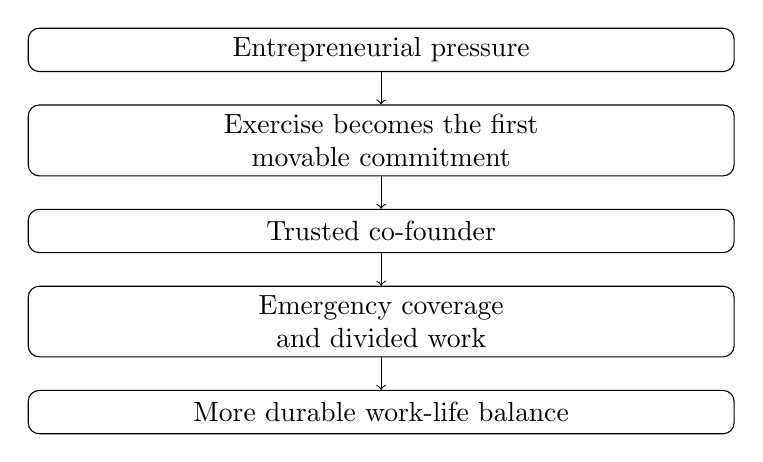
\begin{tikzpicture}
\node[draw, rounded corners, text width=0.72\linewidth, align=center, minimum height=0.55cm] (a) at (0,0) {Entrepreneurial pressure};
\node[draw, rounded corners, text width=0.72\linewidth, align=center, minimum height=0.55cm] (b) at (0,-1.15) {Exercise becomes the first\\movable commitment};
\node[draw, rounded corners, text width=0.72\linewidth, align=center, minimum height=0.55cm] (c) at (0,-2.30) {Trusted co-founder};
\node[draw, rounded corners, text width=0.72\linewidth, align=center, minimum height=0.55cm] (d) at (0,-3.45) {Emergency coverage\\and divided work};
\node[draw, rounded corners, text width=0.72\linewidth, align=center, minimum height=0.55cm] (e) at (0,-4.60) {More durable work-life balance};
\draw[->] (a) -- (b);
\draw[->] (b) -- (c);
\draw[->] (c) -- (d);
\draw[->] (d) -- (e);
\end{tikzpicture}
\end{figure}

The diagram is a conceptual summary of the interview's sequence, not a board reconstruction. No validated lecture screenshot or blackboard figure is available for this segment.

\section{The Co-Founder As Operational Redundancy}

The speaker grounds the recommendation in his own founding experience. He says he could not have built the company without a strong co-partner. The point is not that every founder needs the same personality type beside them. The point is operational: two trusted partners can offload work for each other.

The transcript gives two concrete cases. First, a personal emergency. If one founder has to step away, the other can cover. Second, ordinary division of work. Even without a crisis, the company can move because responsibility is distributed.

\begin{remark}
The claim here is anecdotal but concrete. It does not say that a co-founder guarantees balance. It says that a strong co-founder can make balance more possible by changing how work is carried.
\end{remark}

This is a useful entrepreneurship mechanism. A founder's health is not only protected by private discipline. It can also be protected by the design of the founding team.

\section{Trust, Enjoyment, and Different Skills}

After recommending partnership, the speaker immediately narrows the requirement. Finding somebody you trust is critical. That word carries real weight. Offloading work only helps if delegation is safe. A partner who cannot be trusted does not reduce the founder's burden; he adds a new one.

The second criterion is that the founder should enjoy working with the person. This is not sentimental. Founding a company requires repeated friction, repeated decisions, and repeated coordination. Enjoyment lowers the cost of that repetition.

The third criterion is skill difference. The transcript phrases this as complementary and even non-complementary skills, so the safest reading is that each founder should bring something the other does not have. In business terms, the partnership should expand the company's capacity rather than duplicate the same narrow strength.

\section{A Compact Mechanism}

We can summarize the logic without pretending it is mathematics. The interview gives us a mechanism, not an equation:

\begin{enumerate}
\item Personal health needs durable practices, and exercise is one of the obvious ones.
\item Under entrepreneurial pressure, the founder treats exercise as movable.
\item A movable practice is likely to be postponed when business demands feel urgent.
\item A trusted co-founder changes the structure of the work.
\item Shared coverage makes emergencies less destructive.
\item Divided work makes the ordinary load less concentrated.
\item Trust, enjoyment, and different skills determine whether the partnership actually works.
\end{enumerate}

The important distinction is between an individual remedy and a structural remedy. Exercise belongs to the individual remedy. Co-founder design belongs to the structural remedy. The speaker does not replace one with the other; he lets the first expose the need for the second.

\section{Summary}

The interview's answer moves in three steps. Exercise is the obvious and true practice for personal and mental health. But founders often cut it first because it feels like the most fungible item in the day. The deeper entrepreneurial lesson is that work-life balance can depend on company structure: a trusted co-founder can absorb emergencies, divide work, and bring skills the founder does not have.